\subsection{期望与条件期望}

\subsubsection{离散随机变量的期望}

\begin{definition}[$X$的期望]\label{def:E(x)}
    $X:\Omega\rightarrow S$
    \[
    \EE(X)=\sum_{x\in S}x\PP(X=x)=\EE^{\PP}(X)
    \]
    当此求和绝对收敛

    注:$\EE^{\PP}(X)$ 强调这是在概率测度 $\PP$ 下的期望
\end{definition}

\begin{definition}[$g(X)$的期望]
    $g:\RR\rightarrow \RR$
    \[
    \EE g(X)=\sum_{x\in S}g(x)\PP(X=x)
    \]
    当此求和绝对收敛
\end{definition}

关于 “求和绝对收敛” 的讨论:

\begin{example}\label{exa:expec2prob}
    $\EE(\II_A)=\PP(A), A\in \CF$
\end{example}

\begin{example}\label{exa:expec_of_indica}
    $X$ 是离散随机变量, 由定义\ref{def:discrete_rv}, $X=\sum_{x\in S}x\II_{A_x}$, 其中 $A_x:=\{X=x\}$. $B$ 是任意的, 求$\EE(\II_B X)$
\end{example}

\begin{remark}
对于 $A_x:=\{X=x\}$ 应这样理解, $A_x$ 是样本空间 $\Omega$ 的一个子集, 包含了所有使得 $X(\omega)=x$ 的样本点 $\omega$. 

根据离散随机变量的定义, $X(\omega)=x_k$ 当且仅当 $\omega\in \Lambda_k$. 因此对于每个 $x_k\in S$, 有
\[
A_{x_k}=\{X=x_k\}=\{\omega\in \Omega|X(\omega)=x_k\}=\Lambda_k
\]

所以 $A_x=\{A_{x_k}\}_{k\geq 1}$ 就是离散随机变量的划分

对于 $X=\sum_{x\in S}x\II_{A_x}$ 可以这样理解. 对于每个 $x\in S$, $\II_{A_x}(\omega)$ 是事件 $A_x=\{X=x\}$ 的指示函数

\[
    \II_{A_x}(\omega)=\begin{cases}
        1 & \text{if } X(\omega)=x\\
        0 & \text{if } X(\omega)\neq x
    \end{cases}
\]
\end{remark}

\begin{solution*}
要先求 $\EE(|\II_B X|)<\infty$ 说明期望存在

对 $\forall \omega\in B$
\[
\begin{aligned}
    \II_B X(\omega)&=\II_B(\omega)\sum_{x\in S}(x\cdot \II_{A_x}(\omega))\\
    &=\sum_{x\in S}x\II_{A_x\cap B}(\omega)
\end{aligned}
\]

其中 $\II_{A_x\cap B}$ 也可记为 $\II_{A_x B}$

$\{A_x B,x\in S\}\cup \{B^c\}$ 构成了样本空间 $\Omega$ 的一个划分. 因为 $A_x$ 本身是对 $\Omega$ 的一个划分, 其与 $B$ 的交是对 $B$ 的划分. 并上 $B^c$, 则满足划分的定义\ref{def:partition}

对于 $\omega\in \Omega$, 由划分
\[
\II_B X(\omega)=0\cdot \II_{B^c}(\omega)+\sum_{x\in S}x\II_{A_x\cap B}
\]

\[
\therefore \EE |\II_B X|=\sum_{x\in S}|x|\PP(A_x B)\leq \sum_{x\in S}|x|\PP(A_x)=\EE|X|<\infty
\]

最后一个等号参考期望的定义\ref{def:E(x)}

\[
\EE (\II_B X)=\sum_{x\in S}x \PP(A_x B)=\sum_{x\in S}x \PP(\{X=x\}\cap B)
\]
\end{solution*}

\begin{theorem}
    $\EE(aX+bY)=a\EE X+b\EE Y$
\end{theorem}

离散随机变量有两种表达形式, 如定义\ref{def:discrete_rv}和练习\ref{exa:expec_of_indica}所示

\[
X=\sum_{x\in S}x\II_{\{X=x\}}=\sum_{k\geq 1}x_k\II_{\Lambda_k}
\]

\[
\sum_{x\in S}x\PP(X=x)=\sum_{k\geq 1}\PP(X=x_k)
\]

只有在“求和绝对收敛”(见定义\ref{def:E(x)})的条件下, 等式才成立

\begin{remark}
    \quad 

    \begin{enumerate}
        \item $\sum_{x\in S}$ (1)级数的重排 (2)可和族
        \item $X$是离散随机变量, $g:\RR\rightarrow\RR$, 则 
        \[
        g(X)=\sum_{x\in S}g(x)\II_{\{X=x\}}
        \]
        是一个离散随机变量, 且 $\sigma(g(X))\st \sigma(X)$. 下面说明这个结论

        当 $x_1\neq x_2$ 时可能 $g(x_1)=g(x_2)$, 因此
        \[
        \Pi_X=\{\{X=x\}|x\in S\}\neq \Pi_{g(X)}
        \]
        其实 $\Pi_{g(X)}\st \sigma(\Pi_X)$, 因为对于 $x_1\neq x_2$ 但 $g(x_1)=g(x_2)$ 的情况, 比如在 $\Pi_X$ 上 $x_1,x_2$ 对应的样本空间是 $\Omega_1,\Omega_2$, 但在 $\Pi_{g(X)}$ 上是 $\Omega_1\cup \Omega_2$. 这一项在 $\Pi_X$ 里有, 因为 $\sigma$代数对可列并封闭. 但 $\Omega_1,\Omega_2$ 分别在 $\Pi_{g(X)}$ 上没有. 把 $\sigma$代数理解成信息, 则 $g(X)=y$ 提供的信息是比直接提供 $x$ 的值要少的(在 $g(\cdot)$ 已知的情况下). 

        \item $X\ind Y,\quad g, h:\RR\rightarrow \RR$, 则 $g(X)\ind h(Y)$. 因为 $\sigma(X)\ind \sigma(Y)$, 而 $\sigma(g(X))\st \sigma(X), \sigma(h(Y))\st \sigma(Y)$
        
        如果 $X,Y$ 是连续随机变量, 则对 $g,h$ 有其他要求. 特殊地, 结论3对 $g,h$ 连续时成立. 
    \end{enumerate}
\end{remark}

\begin{theorem}
    (1) $X\ind Y, \EE|X|<\infty, \EE|Y|<\infty$, 则 $\EE(XY)=\EE(X)\EE(Y)$

    (2) $X_1,X_2,\cdots,X_n$ 相互独立, 则 $\EE(X_1\cdots X_n)=\EE X_1\cdots \EE X_n$

    (3) $X\ind Y, g,h:\RR\rightarrow\RR, \EE|g(X)|<\infty, \EE|h(Y)|<\infty$
    \[
    \Rightarrow g(X)\ind h(Y), \EE(g(X)h(Y))=\EE(g(X))\EE(h(Y))
    \]
\end{theorem}

\begin{theorem}\label{thm:thm1.11}
    若 $X\geq 0$ 取整数值, 则 $\EE (X)=\sum_{k\geq 1}\PP(X\geq k)$
\end{theorem}
\begin{proof}
\[
\sum_{k=1}^{\infty}\PP(X\geq k)=\sum_{k=1}^{\infty}\sum_{l=k}^{\infty}\PP(X=l)=\sum_{l=1}^{\infty}\sum_{k=1}^l \PP(X=l)=\sum_{l=1}^{\infty}l\cdot \PP(X=l)=\sum_{l=0}^{\infty}l\cdot \PP(X=l)=\EE(X)
\]
其中第二个等号求和能交换是由于 Fubini 定理.
\end{proof}

\subsubsection{条件期望}

\subsubsection*{$1^\circ$关于“给定集合”的条件期望}

\begin{definition}\label{def:set_con_exp}
    $(\Omega, \CF, \PP), X:\Omega\rightarrow S, A\in \CF, \PP(A)>0, \EE|X|<\infty$, 定义 $X$ 关于 $A$ 的条件期望
    \[
    \begin{aligned}
        \EE(X|A)&:=\sum_{x\in S}\PP(X=x|A)\\
        &=\sum_{x\in S}x\PP_A(X=x)\\
        &=E^{\PP_A}(X)
    \end{aligned}
    \]
\end{definition}

\begin{property}[线性性]\label{prop:linearity1}
$\EE(aX+bY|A)=a\EE(X|A)+b\EE(Y|A)$
\end{property}

证明:(用期望的性质)

\begin{example}
    $\EE(\II_B|A)=1\cdot \PP(B|A)+0\cdot \PP(B^c|A)=\PP(B|A)$
\end{example}

\begin{example}
    $B\ind A\Rightarrow \EE(\II_B|A)=\EE(\II_B)$
\end{example}

\begin{property}
$\EE|X|<\infty, \PP(A)>0, X\ind \II_A\Rightarrow \EE(X|A)=\EE(X)$
\end{property}

证明:

$\because X\ind \II_A, \therefore \{X=x\}\ind A$
\[
\EE(X|A)=\sum_{x\in S}x\PP(X=x|A)=\sum_{x\in S}x\PP(X=x)=\EE(X)
\]
其中
\[
\sum_{x\in S}x\PP(X=x|A)=\sum_{x\in S}x\frac{\PP(\{X=x\}\cap A)}{P(A)}=\EE(X\II_A)/\PP(A)
\]
最后一个等号由例题\ref{exa:expec_of_indica}

至此没有用到独立性, 可以得到以下推论

\begin{corollary}\label{cor:con_exp_indic}
    $\EE(X|A)=\EE(X\II_A)/\PP(A)$
\end{corollary}

\begin{problem}[作业2-1]
$Y$ 在 $A$ 上取常数 $c$, 证明:$\EE(XY|A)=c\EE(X|A)$
\end{problem}

\subsubsection*{$2^\circ$关于“给定划分生成的$\sigma$代数”的条件期望}

\begin{definition}\label{def:part_con_exp}
    设 $\Pi=\series{\Lambda}{k}$ 是 $\Omega$ 的划分, $X$ 为离散随机变量, $\EE|X|<\infty$, 定义
    \[
    \EE(X|\sigma(\Pi))(\omega):=\EE(X|\Lambda_k)
    \]
    当 $\omega\in \Lambda_k$, 即
    \[
    \EE(X|\sigma(\Pi))=\sum_{k\geq 1}\II_{\Lambda_k}\EE(X|\Lambda_k)
    \]
\end{definition}

期望的本质是积分, 现在因为数分里的积分不够用了, 我们要定义新积分, 希望它也能保留原先的好性质

\begin{property}[线性性]
$\EE(aX+bY|\sigma(\Pi))=a\EE(X|\sigma(\Pi))+b\EE(Y|\sigma(\Pi))$
\end{property}

证明:$\omega\in \Lambda_k$, $LHS=\EE(aX+bY|\Lambda_k)=a\EE(X|\Lambda_k)+b\EE(Y|\Lambda_k)$

第二个等号由性质\ref{prop:linearity1}成立. 

\begin{example}
    \[
    \begin{aligned}
        \EE(X|\{\emp,\Omega\})&=\EE(X|\sigma(\Omega))\\
        &\xlongequal{\text{Def \ref{def:part_con_exp}}}\II_{\Omega}\EE(X|\Omega)\\
        &\xlongequal{\text{Def \ref{def:set_con_exp}}, \Omega\ind X}\sum_{x\in S}x\PP(X=x|\Omega)\\
        &=\sum_{x\in S}x\PP(X=x)\\
        &=\EE(X)
    \end{aligned}
    \]
    独立可以理解为:什么信息也没提供
\end{example}

\begin{example}\label{exa:con_exp_indic}
    \[
    \begin{aligned}
        \EE(\II_B|\sigma(A))&=\EE(\II_B|\{A,A^c,\Omega,\emp\})\\
        &=\EE(\II_B|\sigma(A,A^c))\\
        &=\II_A\EE(\II_B|A)+\II_{A^c}\EE(\II_B|A^c)
    \end{aligned}
    \]
    更进一步, 若 $A\ind B$, 由 $\sigma(B)\ind \sigma(A)\rightarrow \sigma(\II_B)\ind\sigma(\II_A)\Rightarrow \EE(\II_B|\sigma(A))=\EE(\II_B)$
\end{example}

可以把这个结果推广:

\begin{property}
$\sigma(X)\ind \sigma(\Pi)$, 则 $\EE(X|\sigma(\Pi))=\EE(X)$
\end{property}

证明:$\Pi_X=\{\{X=x\}|x\in S\}$, 默认 $x$ 不相同

$\sigma(X)=\sigma(\Pi_X)=\{\{X=x\}|x\in S\}$

不妨设 $\Pi=\{\Lambda_k,k\geq 1\}$

则 $\sigma(X)\ind \sigma(\Pi)\Rightarrow \forall x\in S, k\geq 1, \{X=x\}\ind \Lambda_k$

\[
\begin{aligned}
    \EE(X|\sigma(\Pi)) &= \sum_{k\geq 1}\II_{\Lambda_k}\EE(X|\Lambda_k)\\
    &=\sum_{k\geq 1}\II_{\Lambda_k}\sum_{x\in S}x\PP(X=x|\Lambda_k)\\
    &=\sum_{k\geq 1}\II_{\Lambda_k}\sum_{x\in S}x\PP(X=x)\\
    &=\sum_{k\geq 1}\II_{\Lambda_k}\EE(X)\\
    &=\II_{\Omega}\EE(X)\\
    &=\EE(X)
\end{aligned}
\]

\begin{example}\label{exa:extract_known}
    $\EE(X|\sigma(X))=X$
\end{example}

$\sigma(X)$ 作为条件相当于知道了与 $X$ 相关的所有信息, 即提取已知量

证明:$\sigma(X)=\sigma(\Pi_X)$, 其中 $\II_X=\{\{X=x\}|x\in S\}$

\[
\begin{aligned}
    \EE(X|\sigma(X)) &= \sum_{x\in S}\II_{\{X=x\}}\EE(X|X=x)\\
    &=\sum_{x\in S}\II_{\{X=x\}}\EE(X\II_{\{X=x\}})/\PP(X=x)\quad [\text{Cor }\eqref{cor:con_exp_indic}]\\
    &=\sum_{x\in S}\II_{\{X=x\}}\cdot \frac{x\cdot \PP(X=x)+0\cdot \PP(X\neq x)}{\PP(X=x)}\\
    &=\sum_{x\in S}x\II_{\{X=x\}}=X\qed
\end{aligned}
\]

\begin{property}[提取已知量]\label{prt:extract_known}
设 $\Pi=\{\Lambda_k,k\geq 1\}$ 为 $\Omega$ 的划分, $\EE|X|<\infty, \EE|XY|<\infty$, 则当 $\sigma(X)\st \sigma(\Pi)$ 时, 有
\begin{enumerate}
    \item $\EE(X|\sigma(\Pi))=X$
    \item $\EE(XY|\sigma(\Pi))=X\EE(Y|\sigma(\Pi))$
\end{enumerate}
特别地, 取 $X=\II_A, A\in \sigma(\Pi)$, 则
\begin{enumerate}
    \item $\EE(\II_A|\sigma(\Pi))=\II_A$
    \item $\EE(\II_A Y|\sigma(\Pi))=\II_A \EE(Y|\sigma(\Pi))$
\end{enumerate}
\end{property}

证明:只需证 (2), 因为从 (2)$\rightarrow$(1) 即 $Y=\II_{\Omega}$

$X=\sum_{x\in S}x\II_{A_x}$, 其中 $A_x:=\{X=x\}$

(Step 1) $\sigma(X)=\{\sum_{x\in S_X'}A_x|S_X'\st S_X\}$

$\sigma(X)=\{\sum_{k\in J}\Lambda_k|J\st \NN\}$

已知:$\sigma(X)\st \sigma(\Pi)\Rightarrow \exists$一族 $\series{x}{k}$(可能有相同元素), 使得 $X=\sum_{k\geq 1}x_k\II_{\Lambda_k}$, 其中 $\cup_{k\geq 1}\{x_k\}=S_x$ ($S_x$为取值空间)

注:$\Pi$ 是 $\Pi_X=\{A_x|x\in S\}$ 的加细划分

\begin{figure}[H]
    \centering
    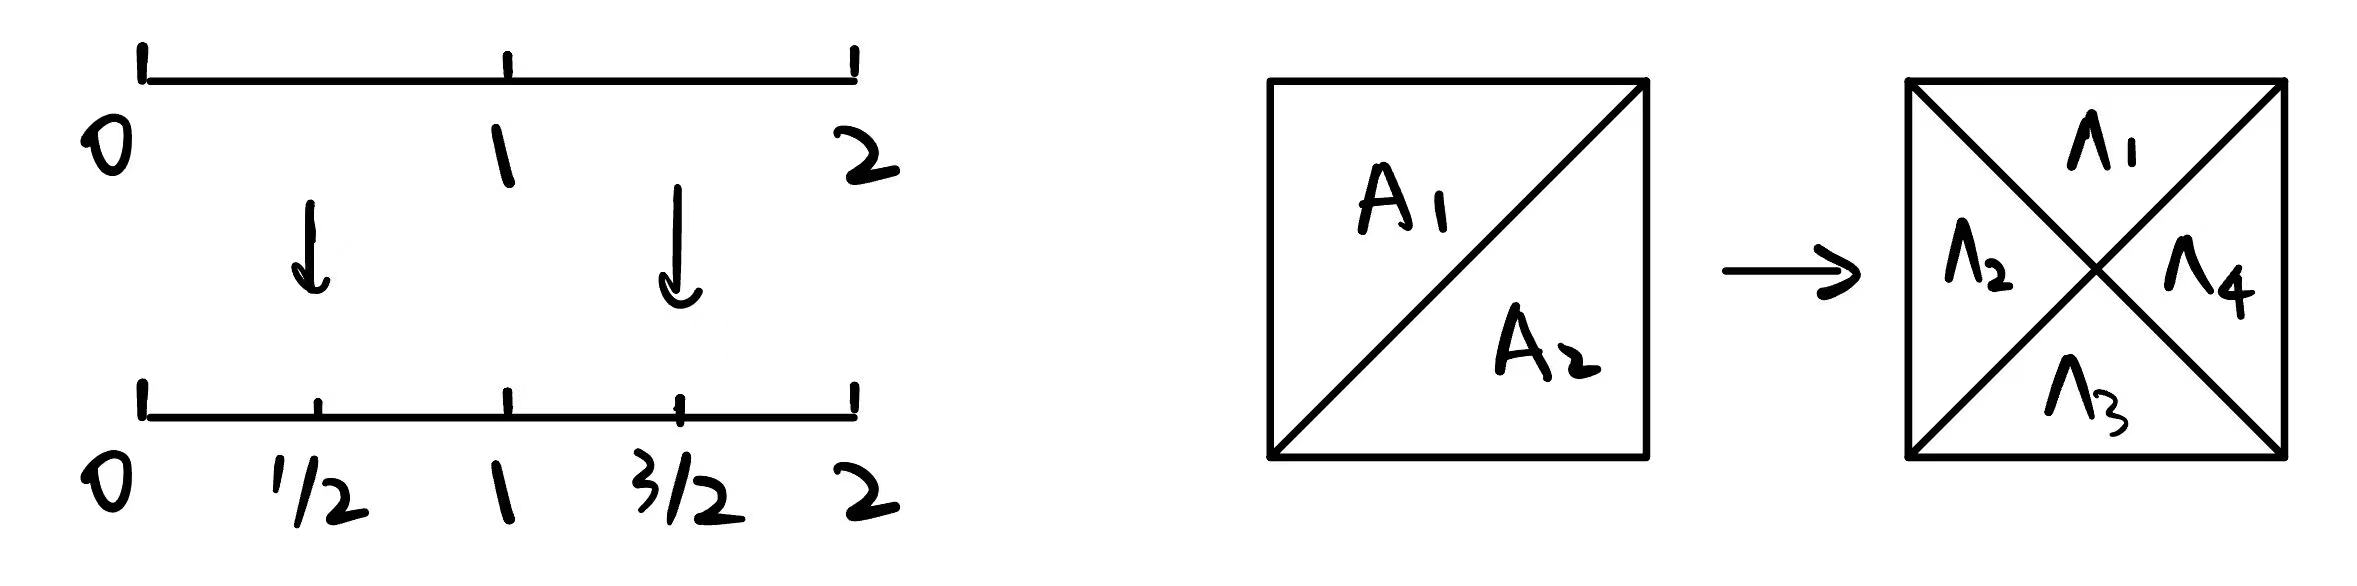
\includegraphics[width=0.8\textwidth]{figures/加细划分.jpg}
    \caption{加细划分}
\end{figure}

(Step 2) 对于 $\omega\in \Lambda_j,\forall j\geq 1$
\[
\begin{aligned}
    \EE(XY|\sigma(\Pi))(\omega) &= \EE(\sum_{k\geq 1}x_k\II_{\Lambda_k}Y|\sigma(\Pi))(\omega)\qquad [X=\sum_{k\geq 1}x_k\II_{\Lambda_k}]\\
    &=\EE(\sum_{k\geq 1}x_k\II_{\Lambda_k}Y|\Lambda_j)\qquad [\sigma(\Pi)\text{定义}]\\
    &=\EE(\sum_{k\geq 1}x_k\II_{\Lambda_k}Y\II_{\Lambda_j})/\PP(\Lambda_j)\qquad [\text{Cor }\eqref{cor:con_exp_indic}]\\
    &=\EE(Yx_j\II_{\Lambda_j})/\PP(\Lambda_j)\qquad [\II_{\Lambda_k}\II_{\Lambda_j}\text{当}\Lambda_k\neq\Lambda_j\text{时}=0]\\
    &=x_j\EE(Y\II_{\Lambda_j})/\PP(\Lambda_j)\\
    &=x_j \EE(Y|\II_{\Lambda_j})\\
    &=X(\omega)\EE(Y|\II_{\Lambda_j})
\end{aligned}
\]

\[
\Rightarrow \EE(XY|\sigma(\Pi))=X\sum_{j\geq 1}\II_{\Lambda_j}\EE(Y|\Lambda_j)=X\EE(Y|\sigma(\Pi))
\]

数学上有种现象叫“法国人的伎俩”, 即把定理当定义用. 严格地讲, 这么做有时会出现存在性和唯一性不满足的问题. 下面介绍一个常被当做定义用的定理:

\begin{theorem}\label{thm:partition_con_exp}
    $\Pi=\{\Lambda_k,k\geq 1\}$ 为 $\Omega$ 的划分,  $\EE|X|<\infty$. 记 $Y:=\EE(X|\sigma(\Pi))=\sum_{k\geq 1}\II_{\Lambda_k}\EE(X|\Lambda_k)$, 则
    \begin{enumerate}
        \item $Y$ 仍是一个离散随机变量, 且 $\EE|Y|\geq \EE|X|<\infty$
        \item $\sigma(Y)\st \sigma(\Pi)$ (记作 $Y\in \sigma(\Pi)$, 即 $Y$ 的所有信息都在 $\sigma(\Pi)$ 里)
        \item $\forall A\in \sigma(\Pi)$, 有 $\EE(Y\II_A)=\EE(X\II_A)$
    \end{enumerate}
\end{theorem}

证明:(1)$E|X|=\sum_{x\in S_x}|x|\PP(X=x)<\infty$

\[
    \EE|Y|=\sum_{k\geq 1}|\EE(X|\Lambda_k)|\PP(\Lambda_k)\geq \sum_{k\geq 1}\sum_{x\in S}|x|\PP(\{X=x\}\cap \Lambda_k)
\]

逻辑上, 现在第一个等号不成立, 但之后 $<\infty$ 一写出来, 之前的所有等号立刻成立, 此处只为书写简便

\[
    \EE|X|=\sum_{x\in S_x}|x|\PP(X=x)=\sum_{x\in S}|x|\sum_{k\geq 1}\PP(\Lambda_k\cap \{X=x\})
\]

我们知道 $\sum_{x\in S}|x|\sum_{k\geq 1}\PP(\Lambda_k\cap \{X=x\})$ 绝对收敛, 若求和次序交换后的 $\sum_{k\geq 1}\sum_{x\in S}|x|\PP(\{X=x\}\cap \Lambda_k)$ 也绝对收敛, 则 $\EE|Y|<\infty$ 得证. 有一个引理可以保证绝对收敛:

\begin{lemma}[\cite{calculus}.P280.推论]\label{lem:abs_convergence}
    从 273-280
\end{lemma}

\begin{corollary}\label{cor:double_exp}
    来自Thm \ref{thm:partition_con_exp}(1).
    \begin{enumerate}
        \item (重期望公式)
        \begin{equation}
\EE|\EE(X|\sigma(\Pi))|=\EE|X|, \EE(\EE(X|\sigma(\Pi)))=\EE(X)
\label{eq:double-exp}
\end{equation}
        \item $|\EE(X|\Lambda_k)|\leq \EE(|X|\mid\Lambda_k), |\EE(X|\sigma(\Pi))|\leq \EE(|X|\mid\sigma(\Pi))$
    \end{enumerate}
\end{corollary}

(2) 由定义, $Y=\sum_{k\geq 1}y_k\II_{\Lambda_k}$, 其中 $y_k:=\EE(X|\Lambda_k)$

记 $S_Y=\cup_{k\geq 1}\{y_k\}$, 注意到, 可能 $\exists i\neq j$, 但 $y_i=y_j$

故 $J_y=\{k|y_k=y\}(y\in S_Y)$ 中个数可能大于1

\[
Y=\sum_{y\in S_Y}y\II_{\sum_{k\in J_y}\Lambda_k}
\]

\[
\{Y=y\}=\sum_{k\in J_y}\Lambda_k\in \sigma(\Pi)
\]

\[
\sigma(Y)\st \sigma(\Pi)\qed
\]

(3) $\EE(Y\II_A)=\EE(\II_A\EE(X|\sigma(\Pi)))$

\[
\begin{aligned}
    \EE(Y\II_A)&=\EE(\II_A\EE(X|\sigma(\Pi)))\\
    &=\EE(\EE(X\II_A|\sigma(\Pi)))\qquad [A\in \sigma(\Pi), \text{性质\eqref{prt:extract_known}}]\\
    &=\EE(X\II_A)\qquad [\text{Cor } \eqref{cor:double_exp}]
\end{aligned}
\]

\subsubsection*{$3^\circ$关于离散随机变量的条件期望}

\begin{definition}
    概率空间 $(\Omega,\CF,\PP)$, $X,Y$ 为离散随机变量, $\EE|X|<\infty$. 定义 $\EE(X|Y)=\EE(X|\sigma(Y))=\EE(X|\sigma(\Pi_Y))$, 称为 $X$ 关于 $Y$ 的条件期望
\end{definition}

注:$\omega=\{Y=y\}\in \Pi_Y$ 或 $Y(\omega)=y$, $\EE(X|Y)(\omega)=\EE(X|Y=y)$

\begin{example}
    $\EE(X|\Pi_{\Omega})=\EE(X|\sigma(\Omega))=\EE(X)$
\end{example}

\begin{example}
    $\II_A\ind \II_B\Rightarrow \EE(\II_A|\II_B)=[\text{Exa\eqref{exa:con_exp_indic}}]\EE(\II_A)$
\end{example}

\begin{example}
    $\EE(X|X)=\EE(X|\sigma(X))=X$[\text{Exa \ref{exa:extract_known}}]
\end{example}

\begin{property}
    假设以下期望、条件期望都有意义
    \begin{enumerate}
        \item $\EE(aX+bY|Z)=a\EE(X|Z)+b\EE(Y|Z)$
        \item $X\ind Y\Rightarrow \EE(X|Y)=\EE(X)$
        \item $\sigma(X)\st \sigma(Z)\Rightarrow \EE(XY|Z)=X\EE(Y|Z)$
        \item $\EE(\EE(X|Z))=\EE(X)$
        \item $|\EE(X|Z)|\leq \EE(|X|\mid Z)$
    \end{enumerate}
\end{property}

\subsubsection*{$4^\circ$关于多个离散随机变量的条件期望}

$\EE(Y|X_1,\cdots,X_n)$

\begin{enumerate}
    \item 由 $X_1,\cdots ,X_n$ 生成的 $\sigma$代数 $\sigma(X_1,\cdots,X_n)$
    \item $:=\EE(Y|\sigma(X_1,\cdots ,X_n))$
\end{enumerate}

怎样生成 $\sigma$代数可以包含 $X_1,\cdots,X_n$ 尽可能多的信息?

直觉是 $\bigcup_{k=1}^{\infty}\sigma(X_k)$, 然而它不一定是 $\sigma$代数, 因为它对可列并不封闭. 

每个 \(\sigma(X_k)\) 是一个 \(\sigma\)代数, 因此它对可列并封闭. 

然而, \(\bigcup_{k=1}^{\infty} \sigma(X_k)\) 只是将每个 \(\sigma(X_k)\) 中的集合简单地并在一起, 并没有保证这些集合的可列并仍然在 \(\bigcup_{k=1}^{\infty} \sigma(X_k)\) 中. 

例如, 假设 \(X_k \in \sigma(X_k)\), 那么 \(X_k\) 在 \(\bigcup_{k=1}^{\infty} \sigma(X_k)\) 中, 但 \(\bigcup_{k=1}^{\infty} X_k\) 可能不在 \(\bigcup_{k=1}^{\infty} \sigma(X_k)\) 中, 因为它可能不属于任何一个单独的 \(\sigma(X_k)\). 问题出在 \(\bigcup_{k=1}^{\infty} \sigma(X_k)\) 缺少 $\{\sigma(X_k)\}_{k\geq 1}$ 交互的部分

怎样把 \(\bigcup_{k=1}^{\infty} \sigma(X_k)\) 变成$\sigma$代数?

\begin{definition}[多个离散随机变量生成的$\sigma$-代数]\label{def:multi_rv_con_exp}
    定义由离散随机变量 $X_1,\cdots,X_n$ 生成的 $\sigma$代数
    \[
    \begin{aligned}
        \sigma(X_1,\cdots,X_n)&:=(X_1,\cdots,X_n)^{-1}(2^{S_1}\times \cdots \times 2^{S_n})\\
        &:=\{\underbrace{(X_1,\cdots,X_n)^{-1}(A_1\times\cdots\times A_n)}_{\text{柱集}}|A_1\times\cdots\times A_n\st \underbrace{S_1\times\cdots\times S_n}_{\text{乘积空间}}\}\\
        &=\left\{\bigcap_{k=1}^{\infty}X_k^{-1}(A_k)|A_k\in 2^{S_k},1\leq k\leq n\right\}
    \end{aligned}
    \]
\end{definition}

\begin{theorem}\label{thm:discrete_rv_partition}
    令 $x_k=\sum_{i\geq 1}x_{k,i}\II_{\Lambda_{k,i}}, 1\leq k\leq n$, 为离散随机变量, 对每一个 $k$, $\Pi_k:=\{\Lambda_{k,i}|i\geq 1\}$ 为 $\Omega$ 的划分, 定义
    \[
    \Pi_{(X_1,\cdots,X_n)}:=\{\Lambda_{1,i_1}\cap\cdots \cap \Lambda_{n,i_n}|i_k\geq 1,1\leq k\leq n\}
    \]
    则
    \begin{enumerate}
        \item $\Pi_{(X_1,\cdots,X_n)}$ 是 $\Omega$ 的划分, 且
        \[
            \sigma(\Pi_{(X_1,\cdots,X_n)})=\left \{\sum_{\substack{(i_1,\cdots ,i_n) \\ \in J_1\times \cdots \times J_n}} (\Lambda_{1,i_1}\cap \cdots \cap \Lambda_{1,i_n})|J_k\st \NN,1\leq k\leq n\right \}
        \]
        \item $\sigma(X_1,\cdots,X_n)=\sigma(\Pi_{(X_1,\cdots ,X_n)})$(即定义\ref{def:multi_rv_con_exp}是有意义的, well-defined, make sense, 良定义)
    \end{enumerate}
\end{theorem}

\begin{problem}[作业2-2]
    证明Theorem \ref{thm:discrete_rv_partition}在 $n=2$ 时成立
\end{problem}

\begin{definition}
    $\EE|Z|<\infty$ 定义
    \[
    \EE(Z|X_1,\cdots,X_n)=\EE(Z|\sigma(X_1,\cdots,X_n)):=\EE(Z|\sigma(\Pi_{(X_1,\cdots,X_n)}))
    \]
\end{definition}

\begin{definition}\label{def:multi_rv_indep}
    $(\Omega,\CF,\PP), Y:\Omega\to S_Y, X_1:\Omega\to S_1,X_2:\Omega\to S_2$ 为离散随机变量, 称 $Y$ 和 $(X_1,X_2)$ 独立, 若 $\sigma(Y)\ind \sigma(X_1,X_2)$. [$\sigma(Y)=Y^{-1}(2^{S_Y}),\sigma(X_1,X_2)=(X_1,X_2)^{-1}(2^{S_1}\times 2^{S_2})$]

    即 $\forall A\st S_Y,B\st 2^{S_1}\times 2^{S_2}, B=B_1\times B_2$, 有 
    \[
    \PP(Y\in A,(X_1,X_2)\in B)=\PP(Y\in A)\PP((X_1,X_2)\in B)
    \]
    其中 $\PP((X_1,X_2)\in B)=\PP(X_1\in B_1,X_2\in B_2)$
\end{definition}

\begin{problem}[作业2-3]
    证明:
    \[
    \begin{aligned}
        Y\ind (X_1,X_2)\Leftrightarrow &\forall y\in S_Y,x_1\in S_1,x_2\in S_2\\
        &\text{有}\PP(Y=y,(X_1,X_2)=(x_1,x_2))\\
        &=\PP(Y=y)\PP((X_1,X_2)=(x_1,x_2))
    \end{aligned}
    \]
\end{problem}

有了上述定义, 可以推广:

\begin{enumerate}
    \item $(Y_1,\cdots,Y_n)\ind (X_1,\cdots,X_n)$
    \item $Y\ind_A (X_1,\cdots,X_n) (A\in \CF,\PP(A)>0)$
\end{enumerate}

\begin{property}\label{prop:pairwise_indep}
    $Y\ind (X_1,X_2)\Rightarrow Y\ind X_1,Y\ind X_2$
\end{property}

证明:在定义\ref{def:multi_rv_indep}中取$B_2=\Omega$

\[
\begin{aligned}
    \PP(Y\in A,X_1\in B_1)&=\PP(Y\in A,X_1\in B_1,X_2\in S_2)\\
    &=\PP(Y\in A)\PP(X_1\in B_1,X_2\in S_2)\qquad [Y\ind (X_1,X_2)]\\
    &=\PP(Y\in A)\PP(X_1\in B_1)
\end{aligned}
\]

注:看到 $\Rightarrow$ 要自然地问, 反过来 $\Leftarrow$ 成立吗?做数学要多问自己一些问题, 即便没有答案

\begin{corollary}
    $(Y_1,\cdots,Y_n)\ind (X_1,\cdots,X_n)\Rightarrow Y_k\ind X_j, 1\leq k\leq m,1\leq j\leq n$
\end{corollary}
\newpage